\documentclass[titlepage, a4paper]{article}
\usepackage[swedish]{babel}
\usepackage[utf8]{inputenc}
\usepackage{color}
\usepackage{graphicx}
\usepackage{etoolbox}
\usepackage{stringenc}
\usepackage{pdfescape}

% Sidformat
\usepackage{a4wide}

% Fixa Appendix-titlar
\usepackage[titletoc,title]{appendix}

% Bättre tabeller
\usepackage{tabularx}

% Bättre bildtexter
\usepackage[margin=10pt,font=small,labelfont=bf,labelsep=endash]{caption}

% Enkelt kommando som låter mig attgöra-markera text
\newcommand{\todo}[1] {\textbf{\textcolor{red}{#1}}}

% Nytt \paragraph låter oss ha onumrerade bitar
\makeatletter
\renewcommand\paragraph{\@startsection{paragraph}{4}{\z@}%
{-3.25ex\@plus -1ex \@minus -.2ex}%
{1.5ex \@plus .2ex}%
{\normalfont\normalsize\bfseries}}
\makeatother

\providecommand{\LIPSlogga}{../mall/logga1.png}
\providecommand{\LIPSdatum}{\today}

%% Headers och Footers
\usepackage{fancyhdr}
\pagestyle{fancy}
\lhead{\includegraphics[scale=0.4]{\LIPSlogga}}
\rhead{\ifdef{\LIPSutfardare}{Utfärdat av \LIPSutfardare \\\LIPSdatum}\LIPSdatum}
\lfoot{\LIPSkursnamn \\ \LIPSdokumenttyp}
\cfoot{\thepage}
\rfoot{\LIPSprojektgrupp \\ \LIPSprojektnamn}

%% Titelsida
\newcommand{\LIPSTitelsida}{%
{\ }\vspace{45mm}
\begin{center}
  \textbf{\Huge \LIPSdokument}
\end{center}
\begin{center}
  {\Large Grupp: \LIPSgrupp}
\end{center}
\begin{center}
  {\Large Redaktör: \LIPSredaktor}
\end{center}
\begin{center}
  {\Large \textbf{Version \LIPSversion}}
\end{center}
\vfill
\begin{center}
  {\large Status}\\[1.5ex]
  \begin{tabular}{|*{3}{p{40mm}|}}
    \hline
    Granskad & \LIPSgranskare & \LIPSgranskatdatum \\
    \hline
    Godkänd & \LIPSgodkannare & \LIPSgodkantdatum \\
    \hline
  \end{tabular}
\end{center}
\newpage
}

% Projektidentitet
\newenvironment{LIPSprojektidentitet}{%
{\ }\vspace{45mm}
\begin{center}
  {\Large PROJEKTIDENTITET}\\[0.5ex]
  {\small
  \LIPSartaltermin, \LIPSprojektgrupp\\
  Linköpings Tekniska Högskola, IDA
  }
\end{center}
\begin{center}
  {\normalsize Gruppdeltagare}\\
  \begin{tabular}{|l|l|p{25mm}|l|}
    \hline
    \textbf{Namn} & \textbf{Ansvar} & \textbf{Telefon} & \textbf{E-post} \\
    \hline
}%
{%
    \hline
  \end{tabular}
\end{center}
\begin{center}
  {\small
    \ifdef{\LIPSgruppadress}{\textbf{E-postlista för hela gruppen}: \LIPSgruppadress\\}{}
    \ifdef{\LIPSgrupphemsida}{\textbf{Hemsida}: \LIPSgrupphemsida\\[1ex]}{}
    \ifdef{\LIPSkund}{\textbf{Kund}: \LIPSkund\\}{}
    \ifdef{\LIPSkundkontakt}{\textbf{Kontaktperson hos kund}: \LIPSkundkontakt\\}{}
    \ifdef{\LIPSkursansvarig}{\textbf{Kursansvarig}: \LIPSkursansvarig\\}{}
    \ifdef{\LIPShandledare}{\textbf{Handledare}: \LIPShandledare\\}{}
  }
\end{center}
\newpage
}
\newcommand{\LIPSgruppmedlem}[4]{\hline {#1} & {#2} & {#3} & {#4} \\}

%% Dokumenthistorik
\newenvironment{LIPSdokumenthistorik}{%
\begin{center}
  Dokumenthistorik\\[1ex]
  %\begin{small}
    \begin{tabular}{|l|l|p{60mm}|l|l|}
      \hline
      \textbf{Version} & \textbf{Datum} & \textbf{Utförda förändringar} & \textbf{Utförda av} & \textbf{Granskad} \\
      }%
    {%
			\hline
    \end{tabular}
  %\end{small}
\end{center}
}

\newcommand{\LIPSversionsinfo}[5]{\hline {#1} & {#2} & {#3} & {#4} & {#5} \\}

% Kravlistor
\newenvironment{LIPSkravlista}{
	\center
		\tabularx{\textwidth}{| p{1.2cm} | p{1.9cm} | X | c |}
			\hline
			\textbf{Krav} & \textbf{Förändring} & \textbf{Beskrivning} & \textbf{Prioritet} \\\hline
}
{
		\endtabularx
	\endcenter
}

\newcounter{LIPSkravnummer}
\addtocounter{LIPSkravnummer}{1}
\newcommand{\LIPSkrav}[4][Krav \arabic{LIPSkravnummer}]{{#1} & {#2} & {#3} & {#4} \stepcounter{LIPSkravnummer}\\\hline}


% Leveranskravlistor
\newenvironment{LIPSleveranskravlista}{
	\center
		\tabularx{\textwidth}{| p{1.2cm} | p{1.9cm} | X | X |}
			\hline
			\textbf{Krav} & \textbf{Förändring} & \textbf{Beskrivning} & \textbf{Deadline}\\\hline
}
{
		\endtabularx
	\endcenter
}

\newcounter{LIPSleveranskravnummer}
\addtocounter{LIPSleveranskravnummer}{1}
\newcommand{\LIPSleveranskrav}[4][Krav \arabic{LIPSkravnummer}]{{#1} & {#2} & {#3} & {#4} \stepcounter{LIPSkravnummer}\\\hline}


% Milstolps-lista
\newenvironment{LIPSmilstolpar}{
	\center
		\tabularx{\textwidth}{| p{1.2cm} | X | l |}
			\hline
			\textbf{Nr} & \textbf{Beskrivning} & \textbf{Datum} \\\hline
}
{
		\endtabularx
	\endcenter
}

\newcounter{LIPSstolpnummer}
\addtocounter{LIPSstolpnummer}{1}
%\newcommand{\LIPSmilstolpe}[3][Krav \arabic{LIPSstolpnummer}]{{#1} & {#2} & {#3} \stepcounter{LIPSstolpnummer}\\\hline}
\newcommand{\LIPSmilstolpe}[3]{{#1} & {#2} & {#3} \\\hline}

% Aktivitets-lista
\newenvironment{LIPSaktivitetslista}{
	\center
		\tabularx{\textwidth}{| p{0.3cm} | X | c | c | c |}
			\hline
			\textbf{Nr} & \textbf{Beskrivning} & \textbf{Beroende av} & \textbf{Timmar} & \textbf{datum} \\\hline
}
{
		\endtabularx
	\endcenter
}

\newcounter{LIPSaktivitetsnummer}
\addtocounter{LIPSaktivitetsnummer}{1}
% \newcommand{\LIPSaktivitet}[4][\arabic{LIPSstolpnummer}]{{#1} & {#2} & {#3} & {#4} \stepcounter{LIPSstolpnummer}\\\hline}
\newcommand{\LIPSaktivitet}[5]{{#1} & {#2} & {#3} & {#4} & {#5}\\\hline}

% Mall för mötesprotokoll
\newenvironment{projektmote}[2]{
  {\ }\vspace{5mm}

  \centerline{\textbf{\Huge #1}}
  \vspace{2mm}
  \centerline{\LARGE #2}
  \vspace{10mm}

  \begin{itemize}
}
{
  \end{itemize}
}

\newcounter{paragrafnummer}
\addtocounter{paragrafnummer}{1}
\newcommand{\paragraf}[1]{\item{\textsection \arabic{paragrafnummer}. {#1}}\addtocounter{paragrafnummer}{1}}

% Mall för Statusrapport
\newenvironment{statusrapport}{
  \center
    \tabularx{\textwidth}{| p{0.4cm} | X | X | p{14.5mm} | p{13.5mm} | p{16.5mm} | p{16.5mm} |}
    \hline
    \textbf{Nr} & \textbf{Aktivitet} & \textbf{Beroenden} & \textbf{Planerad tid} & \textbf{Nedlagd tid} & \textbf{Planerad klar} & \textbf{Beräknat klart} \\\hline
}
{
    \endtabularx
  \endcenter
}

\newcommand{\aktivitetstatus}[7]{{#1} & {#2} & {#3} & {#4} & {#5} & {#6} & {#7} \\\hline}	% Importera generella layout-strukturer

% Information nödvändig för generella layout-strukturer
\newcommand{\LIPSgrupp}{50}
\newcommand{\LIPSredaktor}{Martin Söderén}
\newcommand{\LIPSversion}{0.1}
\newcommand{\LIPSdokument}{Kravspecifikation}
\newcommand{\LIPSdokumenttyp}{Kravspecifikation}
\newcommand{\LIPSgranskatdatum}{-}
\newcommand{\LIPSgranskare}{-}
\newcommand{\LIPSgodkannare}{-}
\newcommand{\LIPSgodkantdatum}{-}
\newcommand{\LIPSkursnamn}{TDDD77}
\newcommand{\LIPSprojektnamn}{PONG}
\newcommand{\LIPSprojektgrupp}{Grupp 50}
\newcommand{\LIPSartaltermin}{VT, 2016}
\newcommand{\LIPSgrupphemsida}{https://gitlab.ida.liu.se/oskjo581/tsea83}
\newcommand{\LIPSkund}{LIU}
\newcommand{\LIPSkundkontakt}{-}
\newcommand{\LIPSkursansvarig}{Anders Nilsson}
\newcommand{\LIPShandledare}{-}

% Dokument-specifika paket
\usepackage{tabularx}
\usepackage{tikz}	
\usepackage{amsmath}
\usepackage{amsfonts}
\usepackage{float}
\usetikzlibrary{shapes, arrows}

\pagenumbering{roman}

\begin{document}

\LIPSTitelsida

\begin{LIPSprojektidentitet}
	\LIPSgruppmedlem{Martin Söderén}{Senior Hardware design engineer}{070 816 32 41}{marso329@student.liu.se}
	\LIPSgruppmedlem{Oskar Joelsson}{Junior Hardware design engineer}{076 185 17 17}{oskjo581@student.liu.se}
	\LIPSgruppmedlem{Jesper Jakobsson}{Hardware design intern}{070 673 25 10}{jesja947@student.liu.se}
\end{LIPSprojektidentitet}

%\newpage
%\tableofcontents	%Innehållsförteckning

\newpage

\begin{LIPSdokumenthistorik}
\LIPSversionsinfo{0.1}{2016-02-16}{Första utkast}{Grupp 50}{}
\end{LIPSdokumenthistorik}

\newpage
\pagenumbering{arabic}	%Påbörja sidnumrering

\section{Inledning}
Pong är ett av de första arkadspelen. Det påminner om tennis då två spelare kontrollerar var sin stapel pch med hjälp av dem så skjuter de en boll frma och tillbaka. Målet med spelet är att man ska få bollen bakom motståndarens stapel och på så sätt få poäng.
\begin{center}
\begin{figure}[H]
    \centering
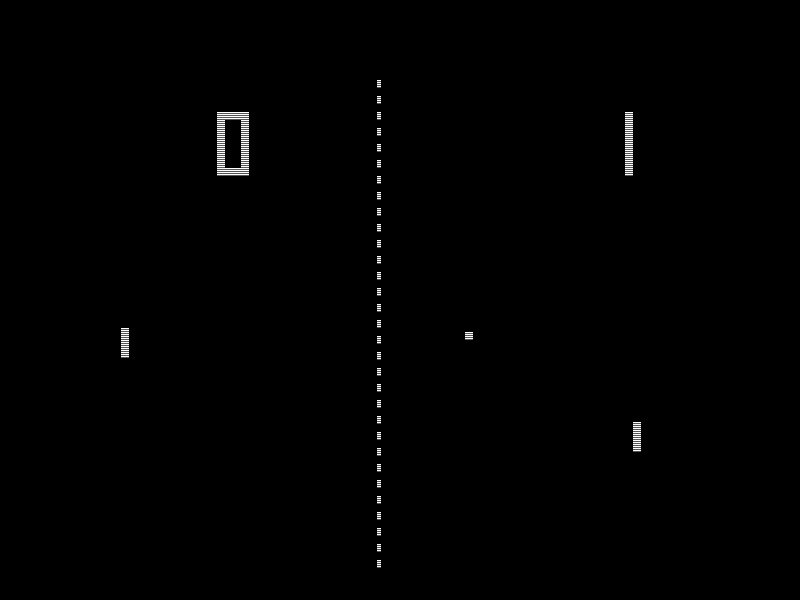
\includegraphics[scale=0.30]{../grafik/Pong.png}
\caption{Pong.}
\label{fig:gui}
\end{figure}
\end{center}

\section{Design}
\subsection{CPU}
\begin{center}
\begin{figure}[H]
    \centering
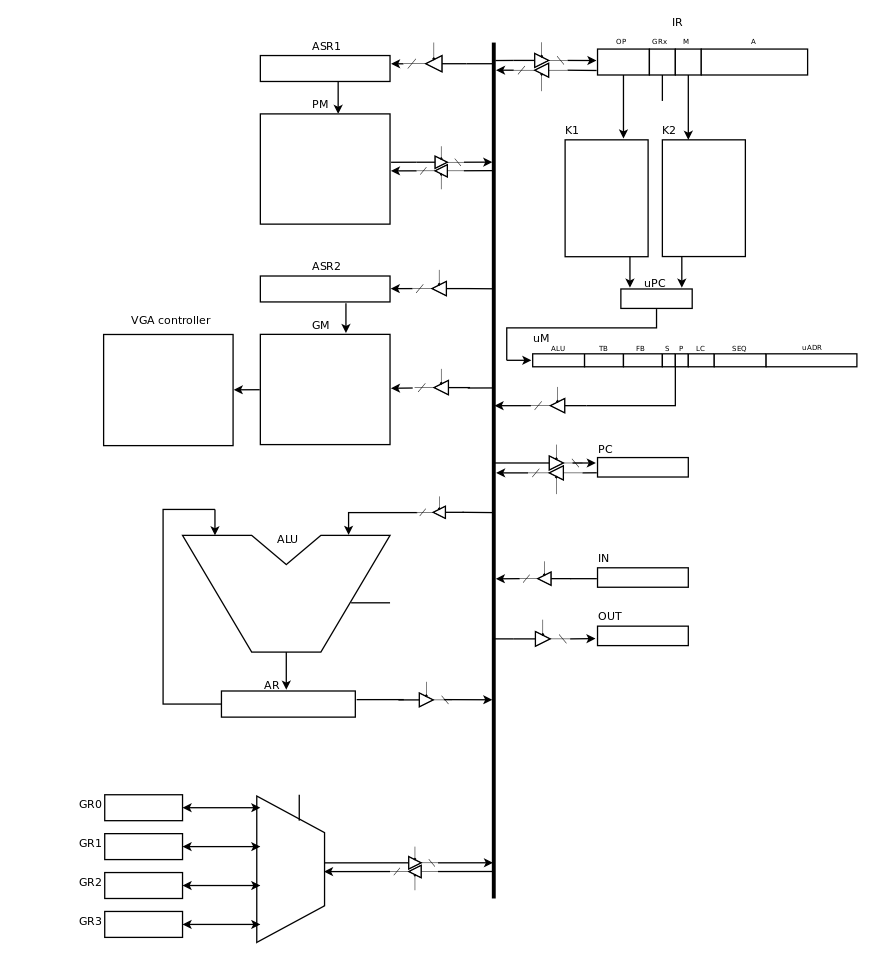
\includegraphics[scale=0.40]{../grafik/overall_design.png}
\caption{Översiktlig design}
\label{fig:gui}
\end{figure}
\end{center}


\subsection{Grafik}
Grafikminnet kommer ett eget minnet med 256 ord à 16 bitar. För att utnyttja grafikminnet maximalt kommer den faktiska upplösningen vara 72x54. Detta leder till att vi behöver 3888 bitar för en bild och vi har 4096 tillgängliga i minnet. För att addressera grafikminnet så har vi en speciell instruktions STOREV som fungerar precis som STORE fast den skriver till grafikminnet. 
\begin{center}
\begin{figure}[H]
    \centering
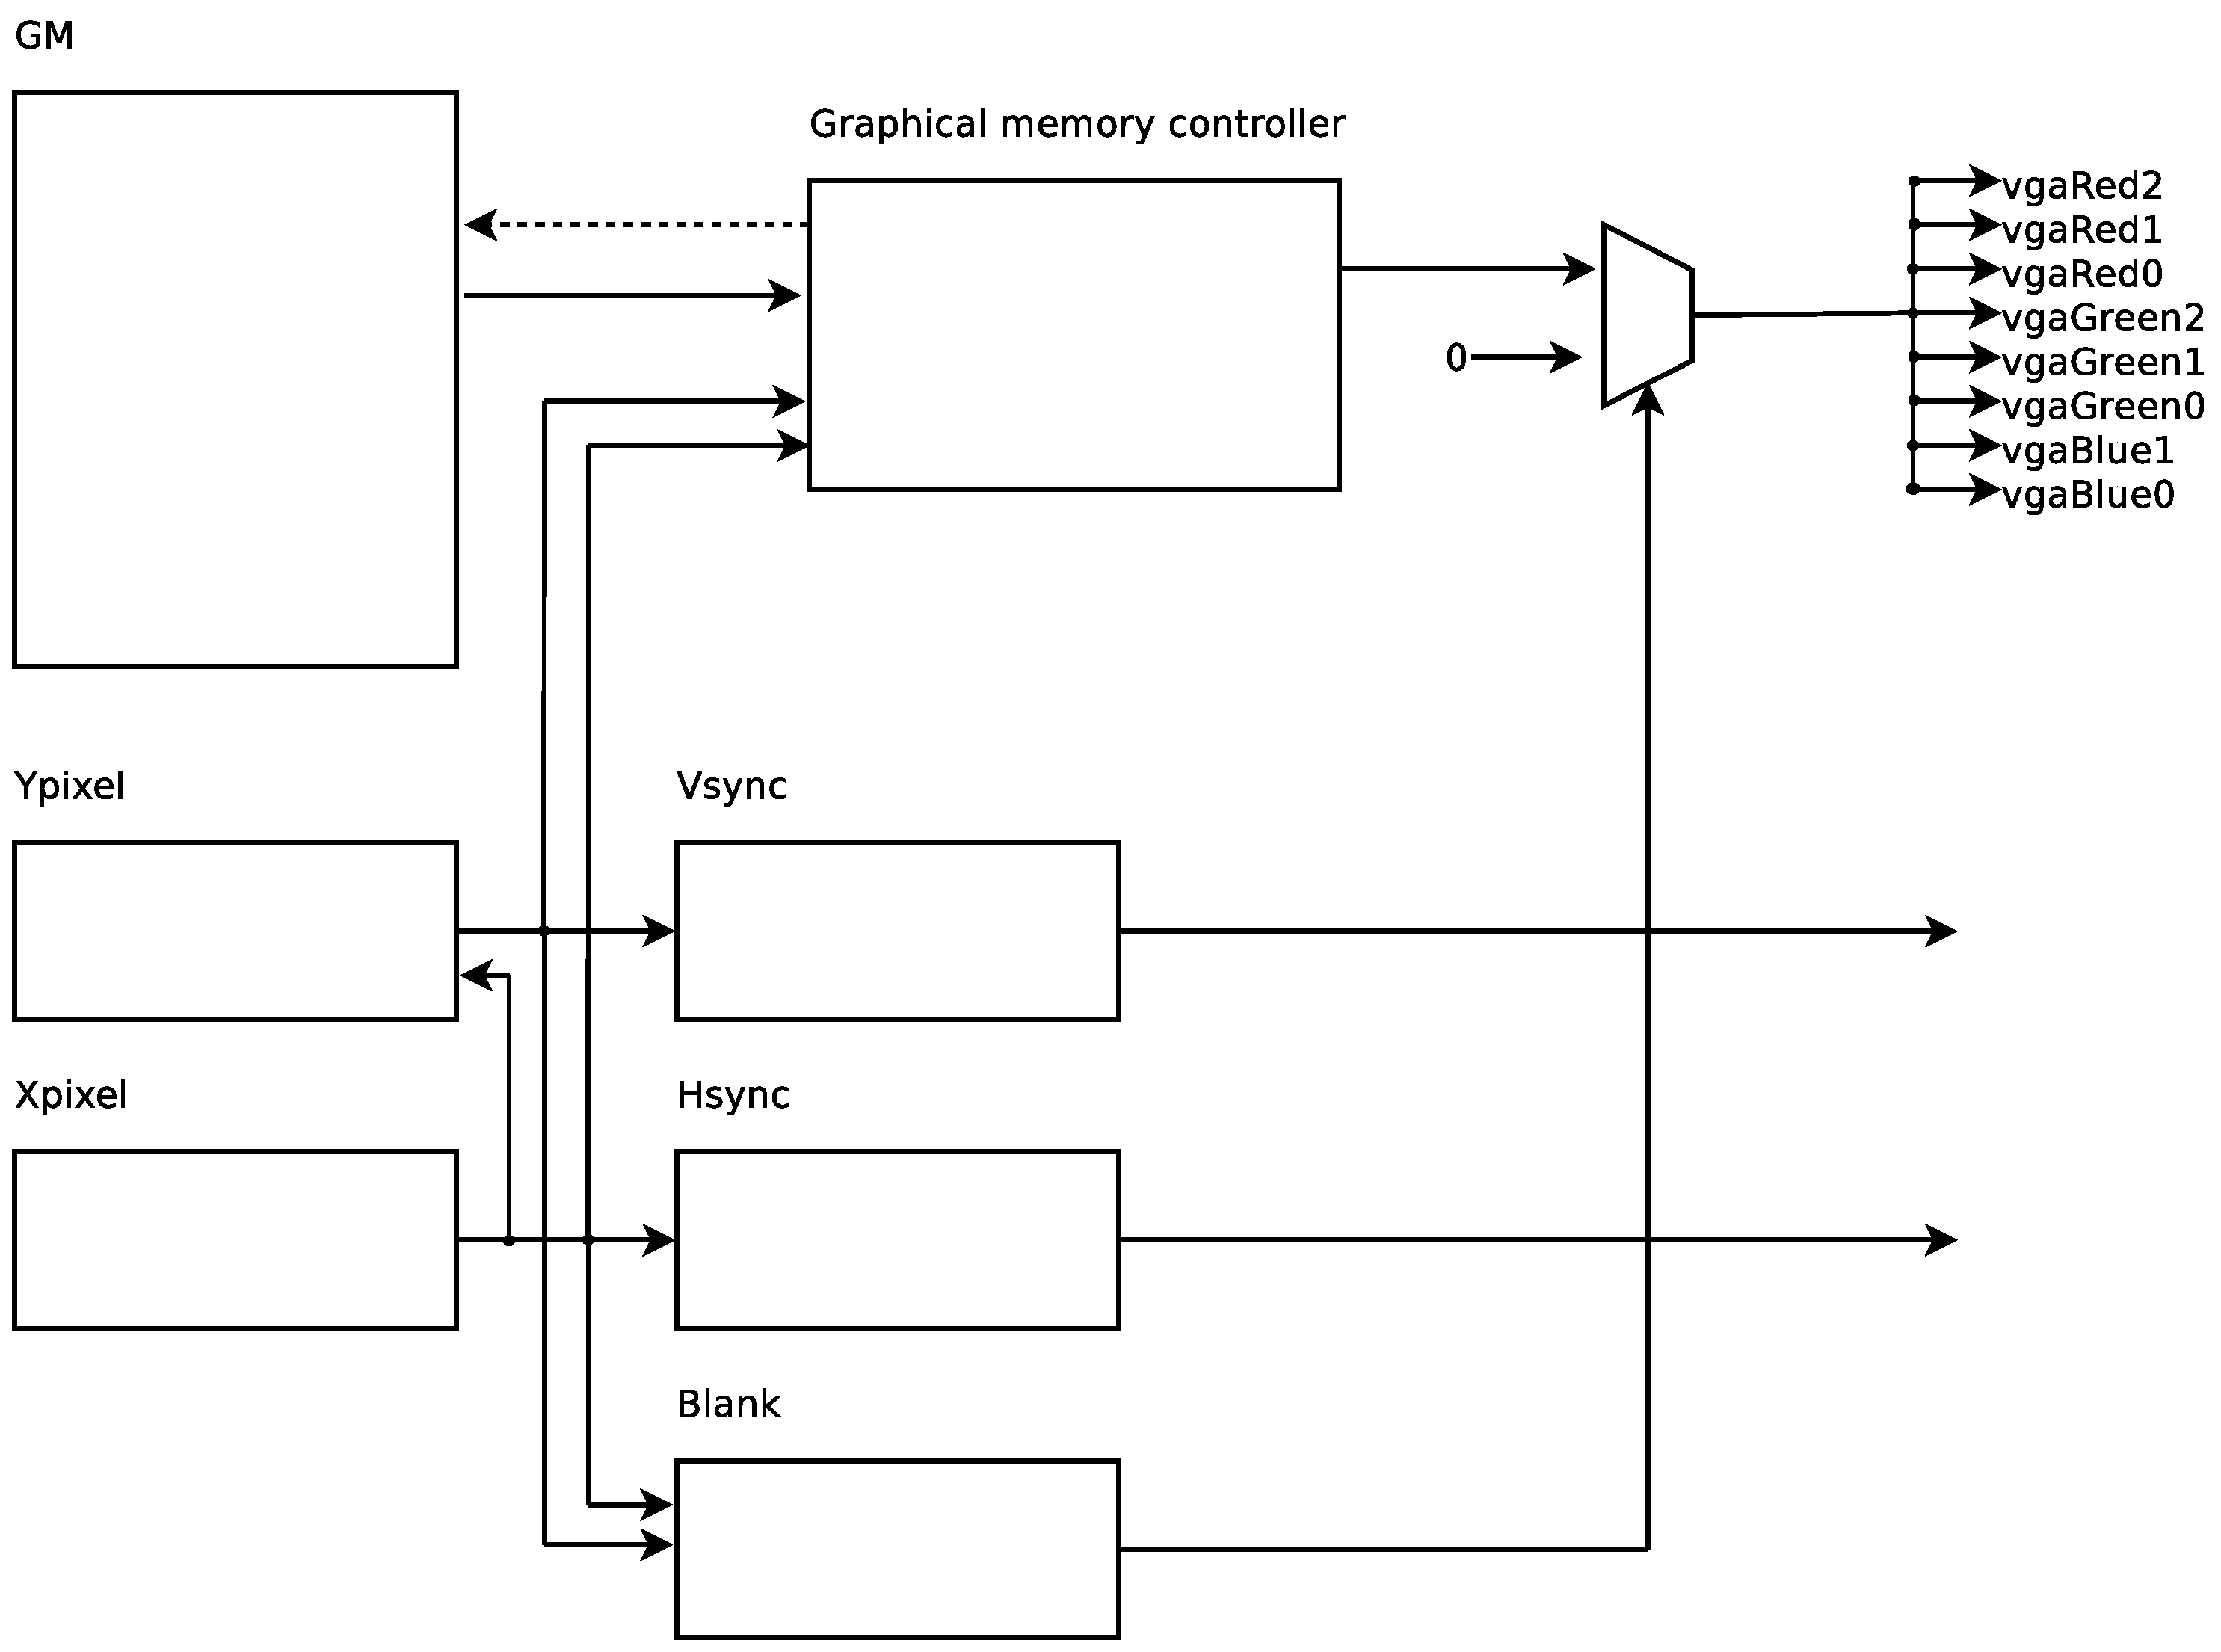
\includegraphics[scale=0.30]{../grafik/graphics.eps}
\caption{Översiktlig design}
\label{fig:gui}
\end{figure}
\end{center} 
\subsection{I/O enheter}
Processorn kommer ha en 8 bitars ingång och en 8 bitars utgång. Instruktionen IN GRx gör att man läser in de 8 bitarna till de 8 minst signifikanta bitarna på register GRx. OUT GRx skriver till utgången. Dessa två portar gör det möjligt att ha en extern 8 bitars ADC och en analog mux för att läsa av flera potentiometers som kommer användas som styrning av staplarna i PONG samt styra hastigheten av bollen. Detta möjliggör även för enklare ljud samt en resetknapp. 
\begin{center}
\begin{figure}[H]
    \centering
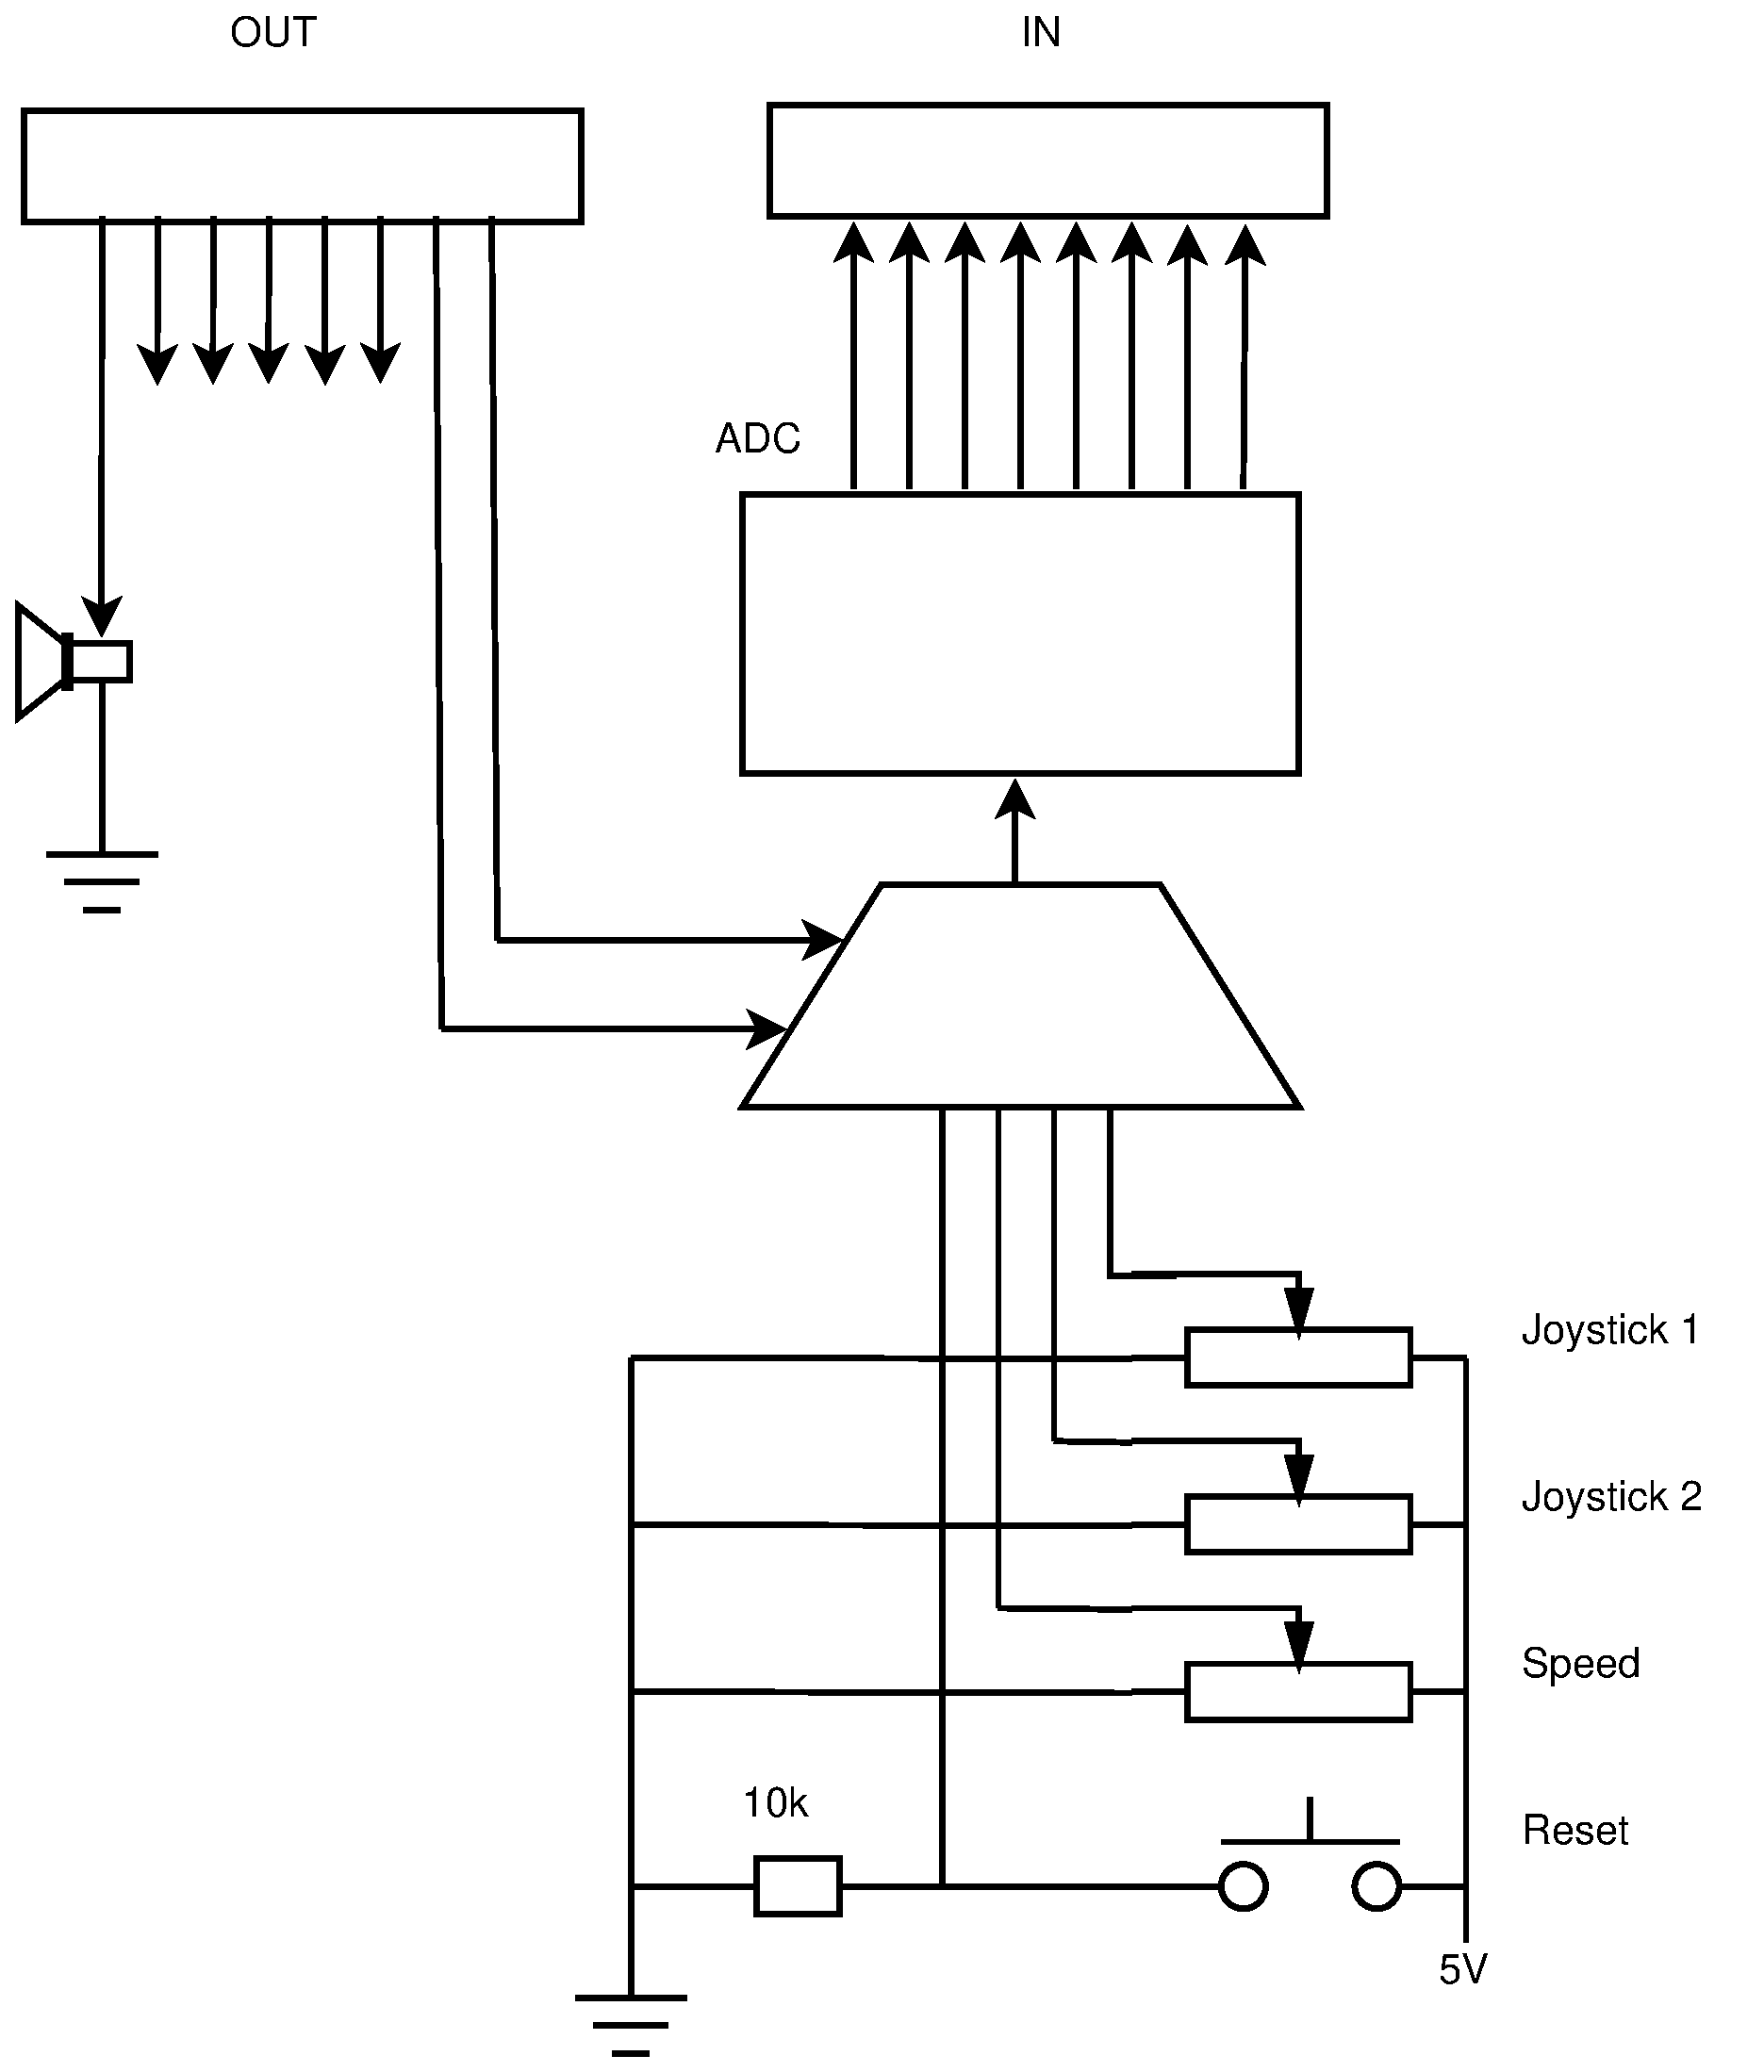
\includegraphics[scale=0.40]{../grafik/io.eps}
\caption{IO design}
\label{fig:gui}
\end{figure}
\end{center}
\subsection{Minnen}
Datorn kommer ha två minnet, dels ett delat programinne och dataminne och sedan ett grafikminne. Primärminnet kommer vara 16 bitar brett och ha 256 ord. Grafikminnet kommer vara likadant.
\subsection{Programmering}
Vi kommer göra en assembler(troligtvis i Python) som från en textfil direkt genererar VHDL kod som vi direkt kan kopiera in i koden för PM.

\section{Kravlista}
Datorn ska vara en egenkonstruerad allmän dator. Med allmän så menas att den ska kunna programmeras om till att utföra andra uppgifter än den som är beskriven här.
\subsection{Skall-krav}
\begin{LIPSkravlista}
\LIPSkrav{Original}{Skärmen ska ha en upplösning på 640x480 med två färger, svart och vitt}{1}
\LIPSkrav{Original}{Skärmen ska ha en uppdateringsfrekvens på 60 Hz}{1}
\LIPSkrav{Original}{Skärmen ska vara en vanlig VGA monitor}{1}
\LIPSkrav{Original}{På spelplanen ska man kunna se båda spelarnas poäng}{1}
\LIPSkrav{Original}{Man ska kunna nollställa spelet med en knapp antingen på joystickarna eller på FPGA-kortet}{1}
\LIPSkrav{Original}{Med joystickarna ska två spelare kunna kontrollera varsin stapel upp och ned}{1}
\LIPSkrav{Original}{Spelet ska ha fungerande kollisions detektion mellan bollen och staplarna}{1}
\end{LIPSkravlista}

\subsection{Bör-krav}
\begin{LIPSkravlista}
\LIPSkrav{Original}{Man ska kunna ställa in hastigheten på bollen på ett enkelt sätt, till exempel en potentiometer och en ADC}{2}
\LIPSkrav{Original}{Bollens riktning efter träff med padeln ska vara en reflektion av bollens infallsvinkeln mot stapeln}{2}
\end{LIPSkravlista}

\end{document}
